%! TeX root = ./informe_final.tex
\chapter{Desarrollo e Implementación}

\section{Configuración del Entorno de Desarrollo Local}
Para asegurar un entorno de desarrollo consistente, aislado y reproducible en la fase de programación, se optó por la contenerización mediante \textbf{Docker} y \textbf{Docker Compose}. Esta metodología permite aislar la aplicación de las particularidades del sistema operativo local (Windows/Linux), empaquetando todas las dependencias del stack Laravel.

La arquitectura de servicios definida en el archivo \texttt{docker-compose.yml} consta de tres contenedores principales interconectados:

\begin{itemize}
    \item \textbf{Servicio App (PHP-FPM):} Construido sobre una imagen de PHP 7.4/8.0, este contenedor procesa la lógica de la aplicación Laravel. Se incluyen extensiones necesarias para el correcto funcionamiento de los reportes PDF y la comunicación con MySQL.
    \item \textbf{Servicio Nginx:} Actúa como servidor web y proxy inverso. Está configurado para servir los archivos estáticos y redirigir las peticiones dinámicas al contenedor de la aplicación.
    \item \textbf{Servicio DB (MySQL 5.7):} Gestiona la persistencia de datos. El volumen de datos está mapeado externamente para garantizar que la información de los turnos no se pierda al reiniciar los contenedores.
\end{itemize}

El uso de redes virtuales (\texttt{turnos\_network}) garantiza una comunicación segura y privada entre los servicios, exponiendo únicamente el puerto 8083 para el acceso externo al sistema.

\section{Estructura general del proyecto}
El proyecto sigue el estándar de \textbf{Laravel 8.x}, organizando el código de manera que la lógica de negocio esté claramente separada de la presentación y los datos. 

\begin{figure}[htbp]
    \centering
    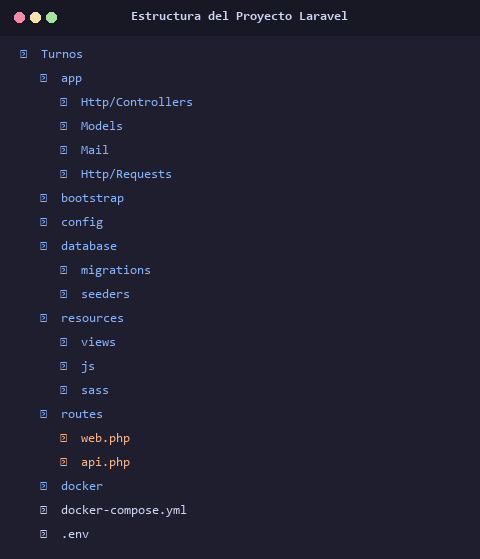
\includegraphics[width=0.55\textwidth]{codigo_tree_proyecto}
    \caption{Estructura general de directorios del proyecto Laravel}
    \label{fig:tree_proyecto}
\end{figure}

Los directorios y componentes principales del proyecto comprenden:

\begin{itemize}
    \item \texttt{app/Models}: Contiene las entidades Eloquent que representan el dominio académico y operativo: \texttt{Turnos\_Dependencias\_Reservas.php}, \texttt{ReservaIntegrante.php}, \texttt{Dependencia.php}, \texttt{Mesas\_Habilitadas.php}, \texttt{Feriado.php}, \texttt{PlantillaEmail.php}, \texttt{Pases.php}, así como los modelos del CMS institucional (\texttt{ProyectoExtension.php}, \texttt{Investigacion.php}, \texttt{MiembroEquipo.php}, \texttt{Instalacion.php}).
    \item \texttt{app/Http/Controllers}: Agrupa los controladores encargados de procesar las solicitudes y coordinar la interacción entre vistas y modelos.
    \item \texttt{database/migrations}: Historial versionado de la estructura de base de datos, garantizando la reproducción consistente del esquema.
    \item \texttt{resources/views}: Plantillas modulares \textbf{Blade}, organizadas en \textit{layouts} maestros para la interfaz pública, el portal del usuario y el panel administrativo.
    \item \texttt{routes/web.php}: Definición centralizada de todas las rutas HTTP del sistema y sus grupos de middlewares asociados.
\end{itemize}

\section{Implementación del Frontend}
El frontend del Sistema de Turnos Académicos ha evolucionado hacia una arquitectura multi-página con un diseño sobrio e institucional, priorizando la claridad de la información y la facilidad de navegación para el visitante y solicitante.

\begin{figure}[htbp]
    \centering
    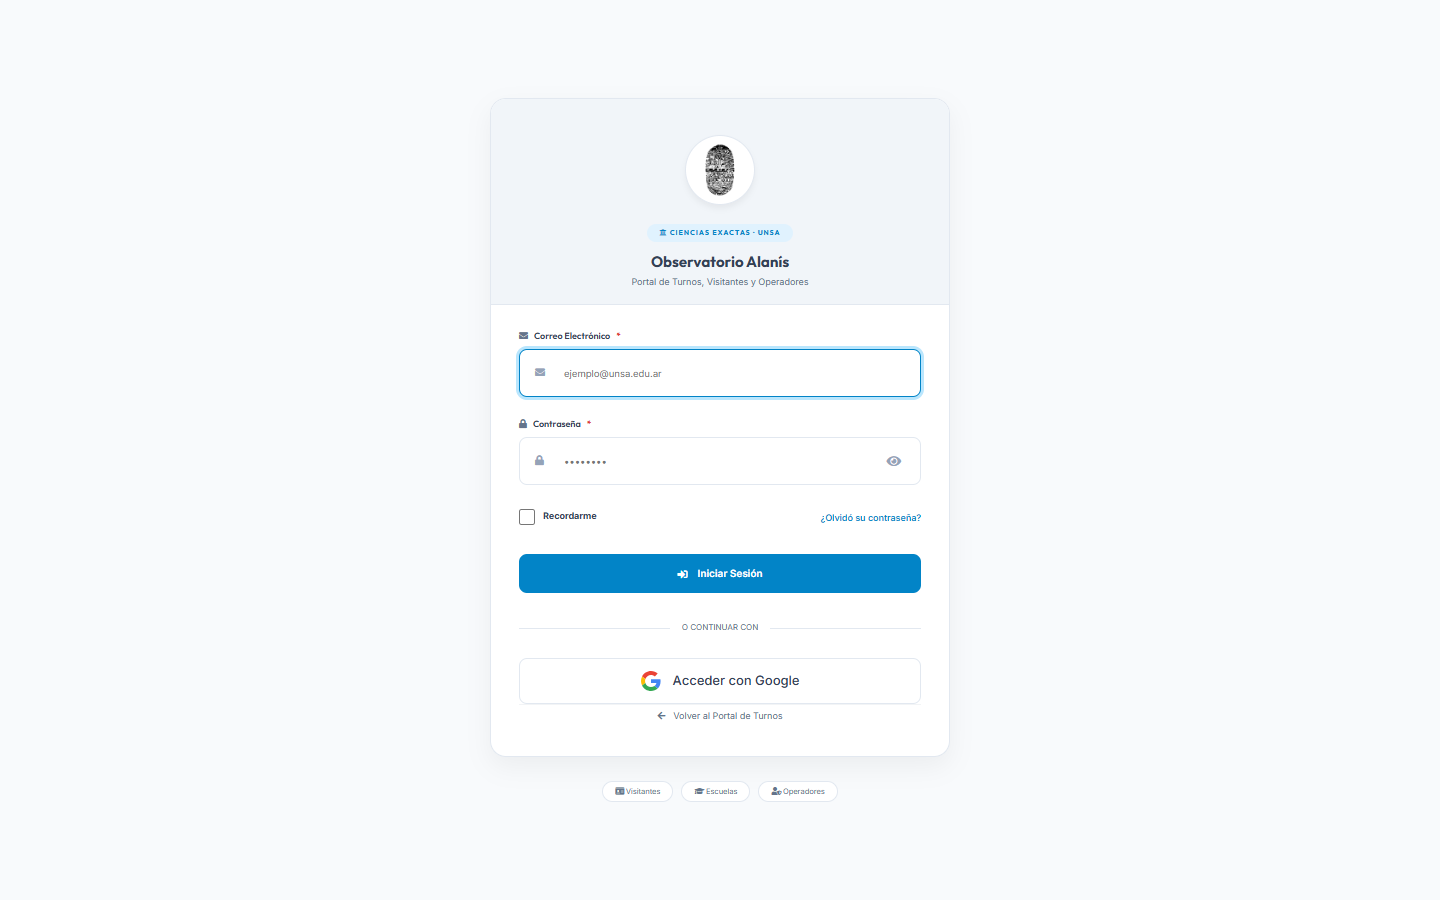
\includegraphics[width=0.85\textwidth]{login_cosmico}
    \caption{Portal de acceso unificado con diseño institucional y autenticación Google Single Sign-On (SSO)}
    \label{fig:login_cosmico}
\end{figure}

Para el inicio de sesión, se implementó una interfaz moderna y limpia, alineada con la identidad visual institucional de la universidad. Además de la autenticación tradicional, se integró el acceso mediante cuentas de Google utilizando el paquete \textbf{Laravel Socialite}, agilizando el registro y acceso de los usuarios a su panel de autogestión.

\subsection{Vistas Blade y Layouts Principales}
La interfaz se organiza alrededor de plantillas maestras en Blade que definen elementos comunes (barra de navegación superior, menús laterales dinámicos, encabezados y pies de página institucionales):
\begin{itemize}
    \item \textbf{Layout Público (\texttt{layouts.frontend}):} Utilizado en la portada, páginas de información y en el asistente de reservas, asegurando una estética sobria adaptada a la UNSa.
    \item \textbf{Layout Administrativo (AdminLTE 4):} Provee un menú lateral colapsable, navegación por migas de pan (\textit{breadcrumbs}), tablas de datos y paneles de tarjetas métricas para el personal del Observatorio y las dependencias.
\end{itemize}

\subsection{Reactividad con Vue.js 2}
En las secciones donde la interacción en tiempo real es crítica, como la selección de horarios en el asistente de reserva, se utilizan componentes de \textbf{Vue.js 2}. Estos componentes consumen endpoints JSON de la API interna para:
\begin{itemize}
    \item Cargar dinámicamente los trámites disponibles al seleccionar una dependencia en el árbol jerárquico sin recargar la página.
    \item Excluir automáticamente del calendario los días inhábiles (feriados y asuetos de la UNSa) consultando \texttt{turnos.getdisableddates}.
    \item Refrescar los horarios libres y cupos restantes de forma reactiva al hacer clic sobre una fecha determinada.
\end{itemize}

\section{Lógica del Backend}
El backend de la aplicación se apoya en los mecanismos nativos de Laravel para garantizar modularidad, seguridad y alto rendimiento.

\subsection{Rutas y Middlewares}
Las rutas del sistema se encuentran agrupadas en \texttt{routes/web.php}, estableciendo una clara separación por niveles de acceso y perfiles de usuario mediante middlewares específicos:

\begin{figure}[htbp]
    \centering
    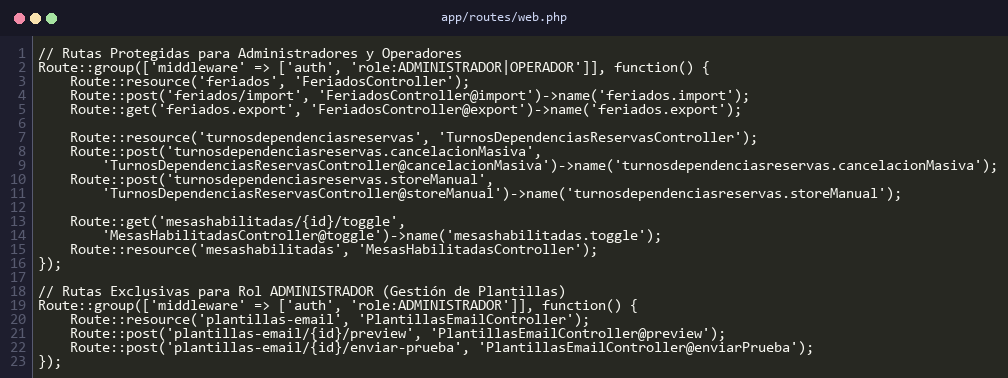
\includegraphics[width=0.92\textwidth]{codigo_rutas_web}
    \caption{Definición de rutas protegidas y filtros de acceso por middleware en \texttt{web.php}}
    \label{fig:codigo_rutas_web}
\end{figure}

\begin{itemize}
    \item \textbf{Rutas Públicas:} Inicio, páginas temáticas, asistente de turnos (\texttt{/turnos}), buscador rápido (\texttt{/turno.buscar}), carga de integrantes (\texttt{/reserva/\{codigo\}/integrantes}) y cancelación pública.
    \item \textbf{Rutas de Autogestión de Turnos (\texttt{middleware('auth')}):} Acceso al panel ``Mis Turnos'' (\texttt{/mis-turnos}) y edición de perfil.
    \item \textbf{Rutas Operativas (\texttt{role:ADMINISTRADOR|OPERADOR}):} Monitoreo diario, bandeja de reservas de turnos, feriados, estadísticas y mesas habilitadas.
    \item \textbf{Rutas Exclusivas de Administrador (\texttt{role:ADMINISTRADOR}):} Gestor web de plantillas de correo transaccional y circuitos.
\end{itemize}

\subsection{Controladores}
Los controladores coordinan la lógica entre las peticiones HTTP, los modelos Eloquent y la presentación.

\begin{figure}[htbp]
    \centering
    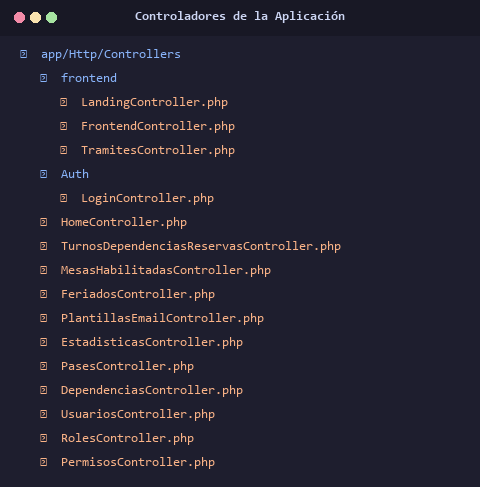
\includegraphics[width=0.55\textwidth]{codigo_tree_controllers}
    \caption{Estructura modular de controladores en \texttt{app/Http/Controllers/}}
    \label{fig:tree_controllers}
\end{figure}

\begin{itemize}
    \item \textbf{Controladores Frontend:} \texttt{LandingController}, \texttt{FrontendController} y \texttt{TramitesController}.
    \item \textbf{Controladores de Operatoria y Gestión:} \texttt{TurnosDependenciasReservasController}, \texttt{MesasHabilitadasController}, \texttt{EstadisticasController} y \texttt{PasesController}.
    \item \textbf{Controladores de Configuración y Seguridad:} \texttt{PlantillasEmailController}, \texttt{FeriadosController}, \texttt{DependenciasController}, \texttt{UsuariosController}, \texttt{RolesController} y \texttt{PermisosController}.
\end{itemize}

\subsection{Modelos y Relaciones con Eloquent}
El dominio de la aplicación se modela mediante entidades Eloquent que encapsulan las relaciones relacionales, mutadores y reglas de integridad.

\begin{figure}[htbp]
    \centering
    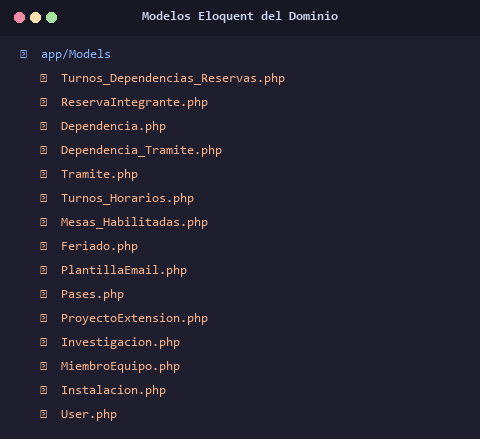
\includegraphics[width=0.55\textwidth]{codigo_tree_models}
    \caption{Modelos Eloquent del dominio en \texttt{app/Models/}}
    \label{fig:tree_models}
\end{figure}

Entre las relaciones más complejas, se destaca el uso de relaciones \texttt{hasOneThrough} e interacciones uno a muchos:

\begin{figure}[htbp]
    \centering
    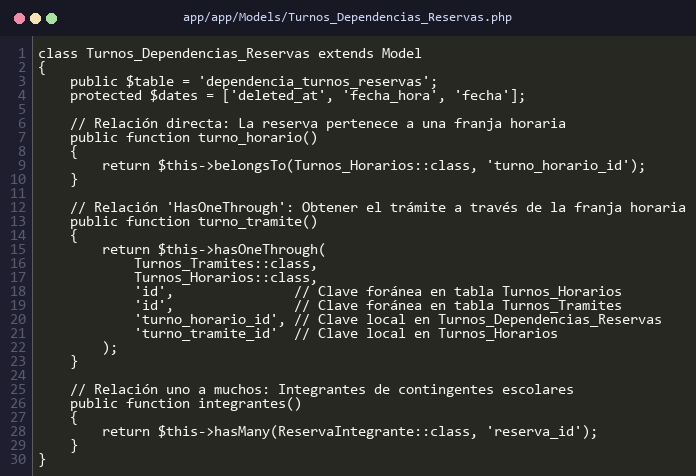
\includegraphics[width=0.92\textwidth]{codigo_modelo_relaciones}
    \caption{Implementación de relaciones Eloquent en \texttt{Turnos\_Dependencias\_Reservas.php}}
    \label{fig:codigo_modelo_relaciones}
\end{figure}

\subsection{Integración de Google Socialite y Enrutamiento por Rol}
Para permitir el acceso ágil de la comunidad universitaria mediante sus cuentas institucionales de Google (\texttt{@unsa.edu.ar}), se implementó el controlador \texttt{LoginController}:

\begin{figure}[htbp]
    \centering
    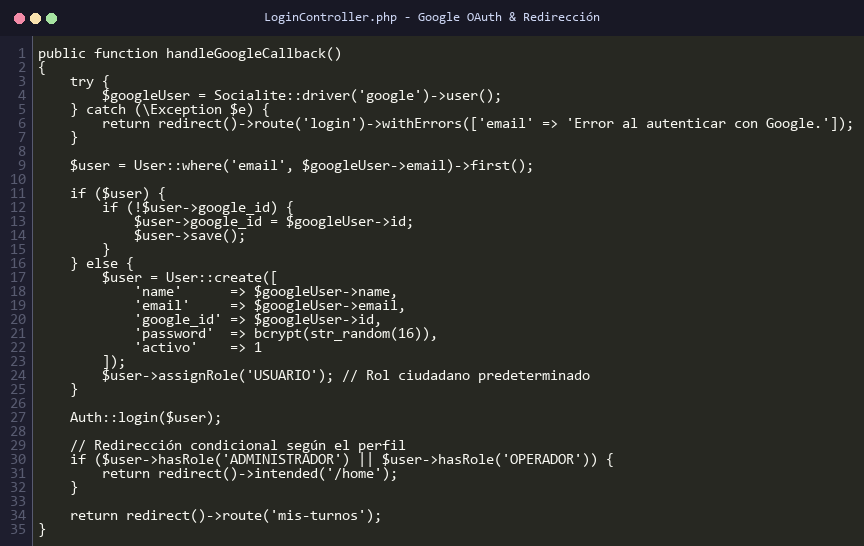
\includegraphics[width=0.92\textwidth]{codigo_socialite}
    \caption{Lógica de autenticación OAuth y redirección condicional por rol en \texttt{LoginController.php}}
    \label{fig:codigo_socialite}
\end{figure}

Si el usuario autenticado posee rol regular (\texttt{USUARIO}), el sistema lo conduce de forma automática a su panel \texttt{mis-turnos}, mientras que los operadores y administradores acceden al panel operativo central.
